\section{Introduction}
\label{sec:intro}

\IEEEPARstart{W}{ith} the continuous growth of satellite missions and sensor technologies, massive volumes of high-resolution and multi-source remote sensing data are now available, providing unprecedented opportunities to monitor the Earth's surface in a timely and comprehensive manner. Accurately identifying and mapping land-cover types is essential for urban planning, precision agriculture, and disaster management \cite{dph26tip}.
 
With the rapid development of Earth observation technologies, a large volume of multi-source remote sensing data has become increasingly accessible. Hyperspectral images (HSIs) capture detailed spectral information across hundreds of contiguous wavelength bands. This rich spectral resolution makes HSI particularly valuable for land cover classification. However, HSI is susceptible to noise and atmospheric interference, which reduces data quality and reliability. To mitigate these challenges, light detection and ranging (LiDAR) and synthetic aperture radar (SAR) data are frequently integrated as complementary sources \cite{hxq26grsl}. LiDAR provides accurate, high-resolution 3D geometric and elevation information, while SAR offers valuable structural, scattering, and dielectric properties regardless of weather and lighting conditions. Consequently, the joint classification of HSI and LiDAR/SAR data has emerged as an effective paradigm to boost classification accuracy and robustness \cite{gf25msf}. Therefore, in this letter, we mainly focus on HSI and SAR/LiDAR joint classification. 

Deep learning-based methods have gained considerable research interest for multi-source remote sensing image joint classification, due to their powerful capability in learning hierarchical feature representations and modeling complex nonlinear relationships  \cite{lxx26tgrs}. By leveraging convolutional neural networks (CNNs) \cite{cnn_vit_backbones} \cite{gcz26tgrs}, Transformers \cite{zyk25grsl} \cite{cui2026mtmixer}, and more recently Mamba architectures \cite{mz26jstars}, these methods can effectively extract discriminative spatial-spectral features from HSI while simultaneously capturing complementary structural and geometric information from SAR and LiDAR data.

\begin{figure*}[!t]
  \centering
  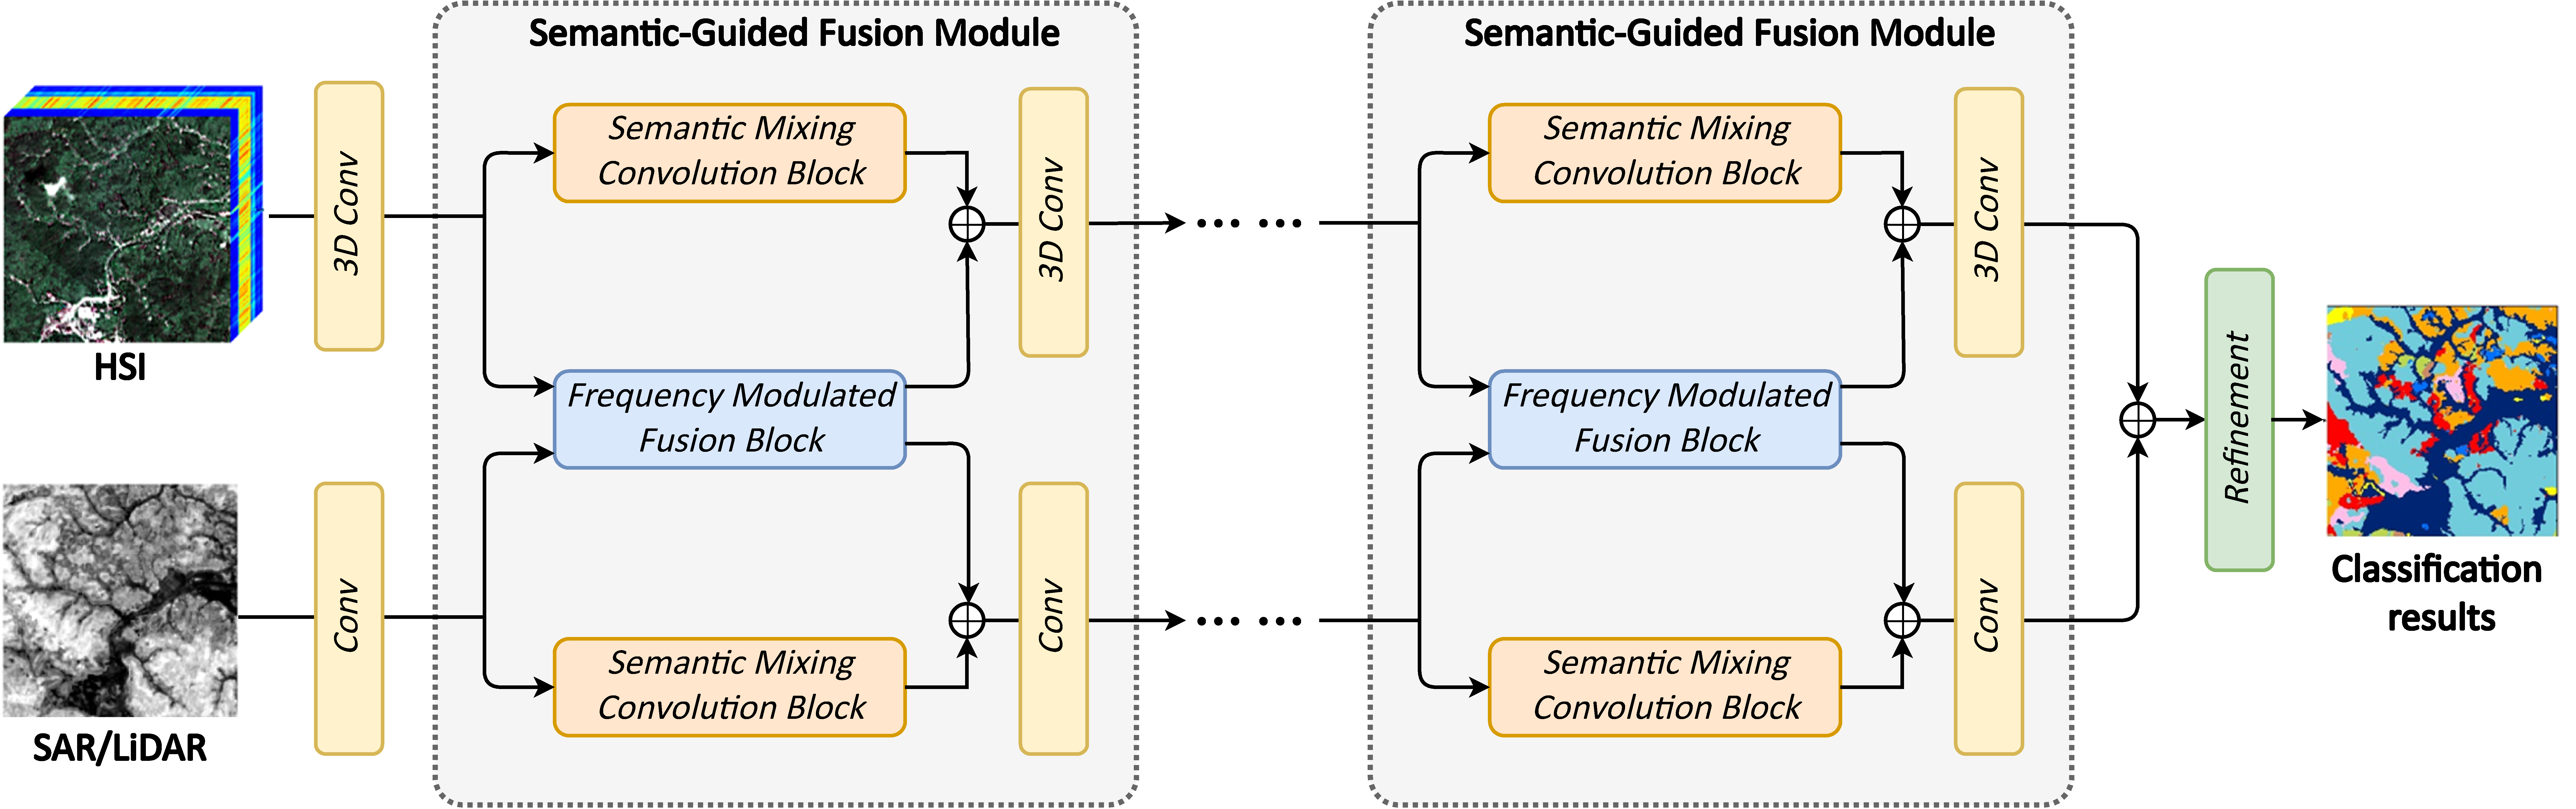
\includegraphics[width=0.8\textwidth]{figures/fig-frame.pdf}
  \caption{Overview of the Semantic-Guided Fusion Network (SGFNet). It adopts a dual-branch hierarchical architecture composed of multiple stacked Semantic-Guided Fusion Modules (SGFMs). Within each SGFM, two Semantic Mixing Convolution Blocks (SMCB) are introduced to model semantic-aware contextual representations. These blocks enhance feature interaction by dynamically integrating global semantic context into local convolution. To further strengthen cross-modal interaction, a Frequency Modulated Fusion Block (FMFB) is inserted between the two branches. It performs frequency-aware feature modulation and adaptive information exchange across modalities.}
  \label{fig-frame}
\end{figure*}

Although existing methods have achieved remarkable classification performance, they still suffer from two limitations: \emph{\textbf{1) Lacking adaptive semantic and contextual representation capability.}} Traditional convolutions use spatially shared and fixed kernels for all spatial locations. Such fixed kernels can hardly adapt to varying semantic structures and content-aware feature distributions. As a result, existing CNN-based methods often fail to effectively capture long-range semantic correlations in complex scenes. \emph{\textbf{2) Slight cross-modal spatial misalignment weakens reliable feature fusion.}} Multi-source remote sensing data acquired by different sensors often suffer from slight spatial misalignment due to inconsistent imaging geometries and sensor characteristics. Although the positional deviations are usually small, local regions and object boundaries may still exhibit structural inconsistencies across modalities. Such misalignment makes direct spatial feature fusion unreliable.

To effectively overcome these limitations, we propose the \textbf{S}emantic-\textbf{G}uided \textbf{F}usion \textbf{Net}work (\textbf{SGFNet}) for multi-source data joint classification. Specifically, to enhance the semantic and contextual feature representations for HSI and SAR/LiDAR data, we propose the \textit{Semantic Mixing Convolution Block (SMCB)}. It dynamically generates semantic-aware convolution kernels according to contextual relationships among feature representations. By enabling position-specific contextual modeling and selectively emphasizing semantically relevant information, the proposed module effectively enhances global semantic dependencies. In addition, we introduce the \textit{Frequency Modulated Fusion Block (FMFB)} to alleviate the slight spatial misalignment between multi-source data. It performs cross-modal feature interaction in the frequency domain rather than directly conducting spatial-domain fusion. Through adaptive frequency-aware modulation, our FMFB effectively enhances complementary information integration and improves the discriminative capability of multi-source feature representations.

Our main contributions are summarized as follows:

\begin{itemize}
  \item \textbf{Feature Enhancement.} We propose SMCB to enhance semantic and contextual feature representations. Unlike conventional convolutions with spatially shared fixed kernels, our SMCB uses semantic-aware dynamic convolution to improve contextual dependency modeling.

  \item \textbf{Cross-Modal Interaction.} We introduce FMFB to alleviate the slight spatial misalignment. By performing adaptive cross-modal interaction in the frequency domain, our FMFB enhances complementary information integration. 
  
  \item \textbf{Experimental Contribution.} Extensive experiments conducted on two benchmark datasets demonstrate that the proposed SGFNet consistently outperforms several state-of-the-art methods. In addition, the source codes will be publicly released to facilitate future research on multi-source data fusion.
\end{itemize}
